\subsection{Módulo de monopolización de hilos por parte de los procesadores}

Tras finalizar el módulo de encendido y apagado de procesadores, nos enfocamos en el desarrollo del módulo de monopolización de hilos por parte de los procesadores. Este módulo introduce la capacidad en el planificador de anclar hilos a una CPU específica, lo que implica que dicho núcleo solo puede encolar y ejecutar los hilos que están asociados a él.\par

\subsubsection{Objetivos}

El objetivo de este módulo es proporcionar al planificador 4BSD la capacidad de anclar hilos a procesadores específicos en cualquier momento durante la ejecución del sistema operativo. Esto permitirá definir políticas de asignación de recursos más precisas y adaptables a las necesidades del sistema.\par

Es muy importante que este módulo, al igual que el desarrollado previamente, pueda ser cargado y activado en tiempo real, sin necesidad de reiniciar el sistema operativo. Esta flexibilidad facilitará su integración con funcionalidades del sistema operativo, como la adaptación dinámica a cambios en la carga de trabajo o la asignación de hilos críticos a núcleos específicos para mejorar el rendimiento, entre otras.\par

\subsubsection{Primera Iteración: Desarrollo del Módulo de Monopolización a través de Políticas en la Red}

Para implementar el módulo de monopolización, se comenzó con una fase de investigación para explorar las posibles estrategias de desarrollo. Inicialmente, se consideró la opción de diseñarlo como un módulo independiente, similar al módulo de encendido/apagado. Sin embargo, se identificó que en última instancia, la decisión del planificador sobre a qué CPU encolar un hilo, estaba estrechamente vinculada a los identificadores de los hilos que se deseaban ejecutar.

Este enfoque nos llevó a entender el problema en términos de políticas para la toma de decisiones a la hora de encolar un hilo. Para implementar estas nuevas políticas, agregamos un mecanismo que permite fijar un hilo a un procesador específico, asegurándonos que dicho procesador no pueda encolar ni ejecutar otros hilos mientras esté monopolizado.

El proceso utiliza un nuevo registro (\textit{pinned\_threads\_per\_cpu}) que rastrea el estado de monopolización de cada uno de los procesadores. Este registro se define como un arreglo de tantos elementos como procesadores en el sistema, en donde que cada elemento almacena el identificador del hilo que se encuentra monopolizando dicho procesador. Así, cuando el planificador debe decidir donde ejecutar el hilo, primero verifica si este se encuentra \textit{anclado} a un procesador específico. Si es así, el hilo se encola en ese procesador para luego ser ejecutado. En caso contrario, el sistema sigue el proceso estándar de asignación a cualquier procesador disponible.

El comportamiento de la elección de procesador desarrollado, se muestra en la Figura \ref{fig:monopolization_resource-choose-cpu}.

\vspace{.50cm}
\begin{figure}[H]
    \centering
    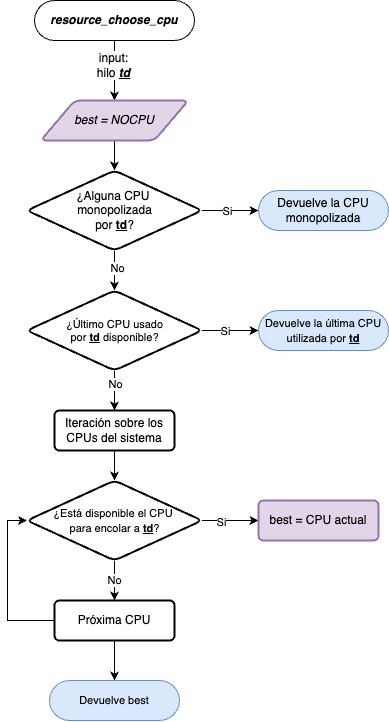
\includegraphics[width=0.35\textwidth]{images/monopolized_choose-cpu.png}
    \caption{Modelo de Monopolización de Hilos por Parte de los Procesadores.}
    \label{fig:monopolization_resource-choose-cpu}
\end{figure}

Junto con el desarrollo de este sistema, también desarrollamos funciones complementarias que permiten alternar el estado de monopolización de los procesadores, liberar un procesador cuando se decida, y verificar si un procesador está ocupado o disponible para un nuevo hilo.

Los detalles técnicos y las implementaciones específicas se encuentran documentados en el Apéndice \ref{appendix:apB}.

\subsubsection{Resultados}

Los resultados del módulo fueron satisfactorios, demostrando que los hilos pudieron monopolizar los procesadores de manera efectiva.\par

Para verificar este comportamiento, realizamos pruebas utilizando una herramienta de monitoreo y un programa de estrés. Estas pruebas consistieron en ejecutar diferentes programas diseñados para mantener hilos activos en los distintos núcleos de las CPUs durante un tiempo prolongado. Inicialmente, se observó el comportamiento global del sistema sin activar el módulo de monopolización. Luego, se seleccionó uno de estos hilos y se lo ancló a un procesador específico. Esto permitió comprobar que el módulo funcionaba correctamente, manteniendo los hilos anclados en un mismo núcleo sin que este pudiera ejecutar otras tareas, lo que confirma la efectividad de la monopolización.\par

Es importante señalar que el módulo no incluyó el caso de la CPU0, ya que, al igual que en pruebas anteriores con el módulo de encendido/apagado, presentaba dificultades para la monopolización debido a su rol en la gestión de tareas administrativas del sistema.\par

Los detalles específicos y un análisis más profundo de los resultados se abordarán en el capítulo de “Análisis de resultados”.\par

\subsubsection{Próximos pasos}

Aunque la implementación de este módulo no genera mejoras inmediatas en el sistema, su potencial radica en su activación bajo demanda, ya sea por señales específicas o por otras partes del kernel. Al igual que en el módulo anterior, su funcionalidad se activa solo cuando es necesario, lo que lo hace útil en escenarios concretos.

Este módulo puede ser particularmente beneficioso en situaciones donde se requiere garantizar la ejecución de tareas críticas en tiempo real o cuando ciertos hilos necesitan acceso exclusivo y preferente a un procesador. Algunos ejemplos en los qeu podría ser beneficioso el módulo son en momentos de interrupciones de hardware a procesadores específicos, asegurando que estos hilos tengan acceso prioritario y minimizando la latencia en la respuesta a eventos de hardware. También podría ser útil en la gestión de dispositivos de almacenamiento de alto rendimiento, donde es crucial que los hilos responsables del acceso a disco mantengan un rendimiento constante.

Otra mejora significante del módulo, sería la de hacer que el mecanismo de anclaje sea más dinámico y flexible. Actualmente, el módulo permite anclar un solo hilo a un solo procesador, pero una posible extensión de esta funcionalidad podría permitir que un procesador ancle múltiples hilos simultáneamente. Esto permitiría una distribución más equilibrada y eficiente de las cargas de trabajo.

Asimismo, se considera la posibilidad de que, en el futuro, se pueda anclar no solo hilos individuales, sino procesos enteros, asegurando que todos sus hilos se ejecuten exclusivamente en ese procesador.